%%
%% 1. Vorlesung 16.10.12
%% 
%% Skript Differentialgeometrie im Wintersemester 12/13
%% Zur Vorlesung von Dr. Grensing am KIT Karlsruhe
%%
%% Mitschrieb und Textsatz von Jan-Bernhard Kordaß.
%%

\section*{"Ubersicht}

\begin{itemize}
\item Mannigfaltigkeiten, Tangentialvektoren
\item Kovariante Ableitung
\item Riemannsche Metriken
\item Krümmung
\item Jacobifelder
\item Satz von Bonnet
\end{itemize}

\section{Differenzierbare Mannigfaltigkeiten}

\begin{dfn*}
  Eine $n$-dimensionale \CmMark{topologische Mannigfaltigkeit} $M$ ist ein topologischer Hausdorff-Raum mit einer abzählbaren Basis der Topologie in dem zu jedem Punkt $p \in M$ eine offene Menge $U$ mit $p \in U$ existiert und ein Hom"oomorphismus $\phi \colon U \to V$ auf eine offene Menge $V \subset \R^{n}$.

% Abbildung 1-1
%\CmPutSvg{1-1-topologische-mf}{8.5cm}
\begin{center}\begin{tikzpicture}[font=\scriptsize]
	\draw[->] (-1.5,0) to[out=20, in=160]node[above,font=\scriptsize]{$\varphi' \circ \varphi^{-1}$} (1.5,0);
	
	\draw[->] (-4,-0.5) -- (-2,-0.5); \draw[->] (-3.75,-0.75) -- (-3.75, 1.25); \node[font=\scriptsize] at (-4, 1.25) {$\R^n$};
	\draw[->] (2,-0.5) -- (4,-0.5); \draw[->] (2.25,-0.75) -- (2.25, 1.25); \node[font=\scriptsize] at (2, 1.25) {$\R^m$};
	
	\node[font=\scriptsize] at (0,2) {$U \cap U' \ne 0$};
	
	\draw (-4.25, 1.75) to[out=70,in=180] (-1.75,3) to[out=300,in=90] (-1.25, 1.25) to[out=180,in=340] (-4.25, 1.75); \node at (-1.25,3) {$M$};
	\filldraw[fill=gray!20] (-2.75,2) circle(0.4); \node[font=\scriptsize] at (-3.25,2.25) {$U$};
	\filldraw[fill=gray!20] (-3,0.25) circle (0.5); \node at (-2.25, 0.5) {$V$};
	\draw[->] (-2.75,1.5) to[out=280,in=80] node[right]{$\varphi$} (-2.75,0.75);
			
	\draw (1.75, 1.75) to[out=70,in=180] (4.25,3) to[out=300,in=90] (4.75, 1.25) to[out=180,in=340] (1.75, 1.75); \node at (4.75,3) {$M$};
	\filldraw[fill=gray!20] (3.55,2.25) circle(0.6); \node[font=\scriptsize] at (2.75,2.25) {$U'$};
		
	\coordinate (ctrl0up) at ($(2.5,-0.25) + 0.2*(0.5,2)$); \coordinate (ctrl0down) at ($(2.5,-0.25) + 0.2*(0,-1.5)$);
	\coordinate (ctrl1down) at ($(3,0.25) - 0.1*(0.5,1)$); \coordinate (ctrl1up) at ($(3,0.25) + 0.1*(0.5,1)$);
	\coordinate (ctrl2down) at ($(3,0.7) - 0.1*(0.5,1)$); \coordinate (ctrl2up) at ($(3,0.7) + 0.1*(0.5,1)$);
	\coordinate (ctrl3down) at ($(4,0.5) + 0.3*(-0.5,1)$); \coordinate (ctrl3up) at ($(4,0.5) - 0.3*(-0.25,1)$);
	\coordinate (ctrl4down) at ($(3.75,-0.3) + 0.2*(0.8,1)$); \coordinate (ctrl4up) at ($(3.75,-0.3) - 0.2*(0.7,0.75)$);
	\begin{scope}
		\fill[gray!20] (2.5,-0.25) ..controls(ctrl0up) and (ctrl1down).. (3,0.25) ..controls(ctrl1up) and (ctrl2down).. (3,0.7) ..controls(ctrl2up) and (ctrl3down).. (4,0.5) ..controls(ctrl3up) and (ctrl4down).. (3.75,-0.3) ..controls(ctrl4up) and (ctrl0down).. (2.5,-0.25); \node at (4.25, 0.5) {$V'$};
		\clip(2.5,-0.25) ..controls(ctrl0up) and (ctrl1down).. (3,0.25) ..controls(ctrl1up) and (ctrl2down).. (3,0.7) ..controls(ctrl2up) and (ctrl3down).. (4,0.5) ..controls(ctrl3up) and (ctrl4down).. (3.75,-0.3) ..controls(ctrl4up) and (ctrl0down).. (2.5,-0.25); \node at (4.25, 0.5) {$V'$};
		\fill[gray] (2,0) circle (1);
		 (2.5,-0.25) ..controls(ctrl0up) and (ctrl1down).. (3,0.25) ..controls(ctrl1up) and (ctrl2down).. (3,0.7) ..controls(ctrl2up) and (ctrl3down).. (4,0.5) ..controls(ctrl3up) and (ctrl4down).. (3.75,-0.3) ..controls(ctrl4up) and (ctrl0down).. (2.5,-0.25); \node at (4.25, 0.5) {$V'$};
	\end{scope}
	\draw  (2.5,-0.25) ..controls(ctrl0up) and (ctrl1down).. (3,0.25) ..controls(ctrl1up) and (ctrl2down).. (3,0.7) ..controls(ctrl2up) and (ctrl3down).. (4,0.5) ..controls(ctrl3up) and (ctrl4down).. (3.75,-0.3) ..controls(ctrl4up) and (ctrl0down).. (2.5,-0.25); \node at (4.25, 0.5) {$V'$};
	\draw[->] (3.5,1.5) to[out=280,in=80] node[right]{$\varphi'$} (3.5,0.75);
\end{tikzpicture}\end{center}

  $\varphi' \circ \varphi^{-1}$ ist ein Hom"oomorphismus offener Mengen des $\R^n$ bzw. $\R^m$. Nach dem Satz von Brouwer (1912) gilt dann $m = n$. Damit ist die Dimension einer zusammenh"angenden topologischen Mannigfaltigkeit eindeutig definiert.\\

  Die Abbildung $\varphi \colon U \to V \subset \R^n$ hei\ss t \CmMark{Karte} von $M$ um $p$, die Menge $U$ hei\ss t \CmMark{Kartengebiet}.\\

  Eine Menge von Karten $\mathcal A = \{(\varphi_{\alpha}, U_{\alpha}) \mid \alpha \in J \}$ hei\ss t \CmMark{Atlas} von $M$, falls $\bigcup_{\alpha \in J}U_{\alpha} = M$.\\

  Ein Atlas $\mathcal A$ von $M$ hei\ss t $C^k$-Atlas, wenn für alle $\alpha, \beta \in J$ mit $U_{\alpha} \cap U_{\beta} \neq \emptyset$ der sogenannte \CmMark{Kartenwechsel}:
  \begin{align*}
    \varphi_{\beta} \circ \varphi_{\alpha}^{-1}\colon \varphi_{\alpha}(U_{\alpha} \cap U_{\beta}) \to \varphi_{\beta}(U_{\alpha} \cap U_{\beta})
  \end{align*}
  ein $C^k$-Diffeomorphismus ist.\\

  % Abbildung 1-2
  %\CmPutSvg{1-2-kartenwechsel}{8cm}
  \begin{center}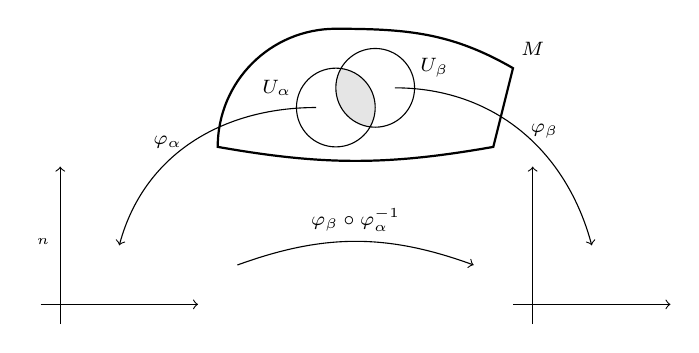
\begin{tikzpicture}[font=\scriptsize]
  	\draw[->] (-1.5,0) to[out=20, in=160]node[above,font=\scriptsize]{$\varphi_\beta \circ \varphi^{-1}_\alpha$} (1.5,0);
	
	\draw[->] (-4,-0.5) -- (-2,-0.5); \draw[->] (-3.75,-0.75) --node[left]{$\R^n$} (-3.75, 1.25);
	\draw[->] (2,-0.5) -- (4,-0.5); \draw[->] (2.25,-0.75) -- (2.25, 1.25);
	
	\draw[thick]  (-0.25, 3) to[out=0,in = 150] (2,2.5) -- (1.75, 1.5) to[out=190,in=350] (-1.75, 1.5) to[out=90,in=180] (-0.25, 3); \node at (2.25,2.75) {$M$};
	
	\begin{scope}
		\clip (0.25,2.25) circle(0.5);
		\clip (-0.25,2) circle(0.5);
		\fill[gray!20] (0,2) circle(1);
	\end{scope}
	\draw (0.25,2.25) circle(0.5) (-0.25,2) circle(0.5); \node at (-1, 2.25) {$U_\alpha$}; \node at (1,2.5) {$U_\beta$};
	
	\draw[->] (-0.5,2) to[out=180,in=75] node[left]{$\varphi_\alpha$} (-3,0.25);
	\draw[->] (0.5,2.25) to[out=0,in=105] node[right]{$\varphi_\beta$} (3,0.25);
  \end{tikzpicture}\end{center}


  Eine Karte $\psi \colon U \to V$ von $M$ hei\ss t \CmMark{verträglich} mit einem $C^k$-Atlas $\mathcal A = \{(\varphi_{\alpha},U_{\alpha}) \mid \alpha \in J\}$ wenn jeder Kartenwechsel
  \begin{align*}
    \varphi_{\alpha} \circ \psi(U \cap U_{\alpha}) \to \varphi_{\alpha}(U \cap U_{\alpha})
  \end{align*}
  ein $C^k$-Diffeomorphismus ist, i.e. $\mathcal A' = \mathcal A \cup \{(\psi, U)\}$ ist ebenfalls ein $C^k$-Atlas.\\

  Die Menge aller mit $\mathcal A$ verträglichen Karten ist ein \CmMark{maxmaler $C^k$-Atlas}. Jeder maximale Atlas enthält alle mit ihm verträglichen Karten. Ein maximaler $C^k$-Atlas hei\ss t auch \CmMark{$C^k$-differenzierbare Struktur}.

\end{dfn*}

\begin{dfn}[differenzierbare Mannigfaltigkeit]
  Eine \CmMark{differenzierbare Mannigfaltigkeit} der Klasse $C^k$ ist eine topologische Mannigfaltigkeit zusammen mit einer $C^{k}$-differenzierbaren Struktur.\\
\end{dfn}

\begin{bsp}
  Einige Beispiele für glatte Mannigfaltigkeiten:
  \begin{enumerate}
  \item $M = \R^n, \mathcal A = \{(\Id_{\R^n},\R^n)\}$
  \item $M \subset \R^n$ offen, $\mathcal A = \{(\imath_{M},M)\}$
  \item $S^1 \subset \R^2$ ist eine eindimensionale $C^{\infty}$-Mannigfaltigkeit:
    \begin{align*}
      \mathcal A = \{(sin t, \cos t) \mid t \in (0,2\pi)\}
    \end{align*}

    % Abbildung 1-3
    \CmMarginSvg[-2cm]{1-3-karten-der-s1}{3cm}

    ist offen in $S^1$ und
    \begin{align*}
      \varphi \colon (\sin t, \cos t) \mapsto t
    \end{align*}
    ist ein Hom"oomorphismus
    \begin{align*}
      \varphi' \colon U' = \{(\sin t, \cos t) \mid t \in (-\pi,\pi)\} \to (-\pi,\pi)
    \end{align*}
    ebenfalls. $\mathcal A = \{(\varphi, U), (\varphi',U')\}$ ist ein Atlas von $S^1$, denn $U \cup U' = S^1$.
    \begin{align*}
      & \varphi' \circ \varphi^{-1} \colon \varphi(U \cap U') \to \varphi'(U \cap U')\\
      & (0,\pi)\cup(\pi,2\pi) \to (-\pi,0)\cup(0,\pi), t \mapsto \begin{cases}
        t & 0 < t < \pi\\
        t-2\pi & \pi < t < 2\pi
      \end{cases}
    \end{align*}

  \item Jeder reelle Vektorraum endlicher Dimension ist in kanonischer Weise eine $C^{\infty}$-Mannigfaltigkeit.\\
    Wähle eine Basis $\{v_1, \ldots, v_n\}$ von $V$. Diese definiert mit
    \begin{align*}
      \varphi\left(\sum\lambda_iv_i\right) = (\lambda_1, \ldots, \lambda_n)
    \end{align*}
    eine Bijektion auf $\R^n$. Damit erhält man eine globale Karte von $V$.
    Der zugehörige Atlas hängt nicht von der Wahl der Basis ab, denn ist $\{w_1, \ldots, w_n\}$ eine weitere Basis von $V$ und $\psi(\sum \lambda_iw_i) = (\lambda_1, \ldots, \lambda_n)$ eine weitere Karte, so ist $\varphi \circ \psi^{-1}$ als Endomorphismus des $\R^n$ schon $C^{\infty}$.

  \item $S^n = \{(x^0, x^1, \ldots, x^n) \mid \sum_{i = 0}^n(x^{i})^2 = 1\}$.\\

    %% Abbildung 1.4
    \CmMarginSvg{1-4-s3-sphaere}{3.5cm}

    Betrachte den Nordpol $N = (1,0,\ldots,0)$ und den Südpol $S = (-1,0,\ldots,0)$ und die Abbildung
    \begin{align*}
      & \varphi \colon U = S^{n}\setminus\{N\} \to \R^n, x \mapsto \left(\frac{x^1}{1-x^0}, \ldots, \frac{x^{n}}{1-x^0}\right),\\
      & \psi \colon U' = S^{n} \setminus \{S\} \to \R^n, x \mapsto \left(\frac{x^1}{1+x^0}, \ldots, \frac{x^n}{1+x^0}\right)
    \end{align*}

    Aufgabe: Zeige, dass $(\varphi, U), (\psi, U')$ einen $C^{\infty}$-Atlas auf $S^n$ definiert.

  \end{enumerate}
\end{bsp}

\begin{dfn}[Differenzierbare Abbildungen]
  
% Abbildung 1-5
\CmPutSvg{1-5-glatte-abb}{9cm}

Eine stetige Abbildung $f \colon M \to N$ zwischen glatten Mannigfaltigkeiten $M$ und $N$ hei\ss t \CmMark{glatt} ($C^{\infty}$-differenzierbar), wenn es zu jedem $p \in M$ Karten $(\varphi, U)$ in $M$ um $p$ und $(\varphi', U')$ in $N$ um $f(p)$ gibt, so dass $\acute{\varphi} \circ f\circ\varphi^{-1}$ glatt ist.\\

Die Menge aller glatten Abbildungen von $M$ nach $N$ wird $C^{\infty}(M,N)$ genannt.

\end{dfn}

\textbf{Konvention}: Ab jetzt seien zunächst alle Mannigfaltigkeiten, wie auch alle Abbildungen als glatt vorrausgesetzt.

\begin{bem}
  Da Kartenwechsel $C^{\infty}$ sind, gilt obige Bedingung automatisch für alle Karten von $M$ und $N$ (evtl. nach Einschränkung).
\end{bem}

\begin{bsp}
  Es folgen zwei Beispiele für diffenrenzierbare Abbildungen:
  \begin{enumerate}
  \item $(\varphi,U) \in \mathcal A \Rightarrow \varphi \in C^{\infty}(U,\R^n)$, denn
    \begin{align*}
      \Id_{\R^n}\circ \varphi \circ \varphi^{-1} = \varphi \circ \varphi^{-1} \in C^{\infty}.
    \end{align*}
  \item $f \in C^{\infty}(M,N), \ g \in C^{\infty}(N,P) \Rightarrow g \circ f \in C^{\infty}(M,P)$, denn
    \begin{align*}
      \varphi_p \circ g \circ f \circ \varphi^{-1}_m = (\varphi_p \circ g \circ \varphi_n^{-1}) \circ (\varphi_n \circ f \circ \varphi_m^{-1}) \in C^{\infty}.
    \end{align*}
  \end{enumerate}
\end{bsp}

\begin{dfn}[Diffeomorphismus]
  Eine Abbildung $f \colon M \to N$ hei\ss t \CmMark{Diffeomorphismus}, wenn $f$ bijektiv ist und $f$, sowie $f^{-1}$ $C^{\infty}$-Abbildungen von $M$ nach $N$ sind. Insbesondere haben $M$ und $N$ in diesem Fall dieselbe Dimension.\\

Die Menge der Diffeomorphismen von $M$ nach $N$ wird mit $\Diff(M,N)$ bezeichnet. Die Menge der Diffeomorphismen von $M$ nach $M$ wird mit $\Diff(M)$ bezeichnet. $(\Diff(M), \circ)$ ist eine Gruppe.

\end{dfn}

%%% Local Variables: 
%%% mode: latex
%%% TeX-master: "../skript-diffgeom"
%%% End: 
